\section{An "Explosive" Transition}
In this paper we are going to take a deeper look into a specific type of percolation called explosive percolation, where the underlying concept is that the onset of percolation is delayed until a certain point where it then occurs at an accelerated rate.
This occurs when the underlying evolution process works in such a way that the largest cluster size $|C|$ is controlled.
We can think of a graph where multiple clusters might evolve separately without merging.
Collectively they take up a large portion of the graph but there isn't a percolating cluster yet due to the lack of connections between the them.
If at some point these clusters do begin to connect then the graph transitions to the percolating state.
For certain evolution processes it has been heavily debated whether or not the phase transition is continuous or not, so the aim of the next section is to summarize what we know to this point regarding the nature of the transition for said processes.









\subsection{A Selective Process}
This all started in the year 2000 when Dimitris Achlioptas brought forth an interesting take on adding edges to a random graph.
The basic question was what would happen if instead of randomly adding an edge at each step like in the ER model, one evaluated two edges $\{e_1, e_2\}$ and then added one edge and discarded the other according to some selection criteria.
This process of evaluating $m \ge 2$ edges at each step is referred to as an Achlioptas process.
In the next few sections we will see how a small change to the way edges are added can have a big impact on the evolution of the system.









\subsection{The First Look}
In 2001 Tom Bohman and Alan Frieze were the first to design and analyze an Achlioptas process in their paper "Avoiding a Giant component" \cite{BF}, which laid out the Bohman-Frieze (BF) model for delaying the appearance of a giant cluster.
At each step edge $e_1$ is added and $e_2$ discarded if $e_1$ connects two clusters of size smaller than or equal to $K$, if not $e_2$ is added and $e_1$ discarded.
In their paper they took $K = 1$, thus the algorithm favors connecting isolated nodes rather than connecting clusters containing two or more nodes.
This is known as a "bounded-size" rule which essentially views all clusters of size greater than $K$ as equivalent.
They were able to show that this method (using $K = 1$) leads to a delayed onset of percolation when compared to the ER model.
This can be seen in Fig. \ref{fig:ER_BF_transition} where the order parameter for the BF model remains smaller than for the ER model, but a little after $r = 0.5$ it begins to rise at a faster rate than in the ER model, eventually overtaking the ER model.
It has been hypothesized that all bounded-size rules produce exhibit continuous phase transitions \cite{Spencer_Wormald}.

\begin{figure}[H]
	\centering
	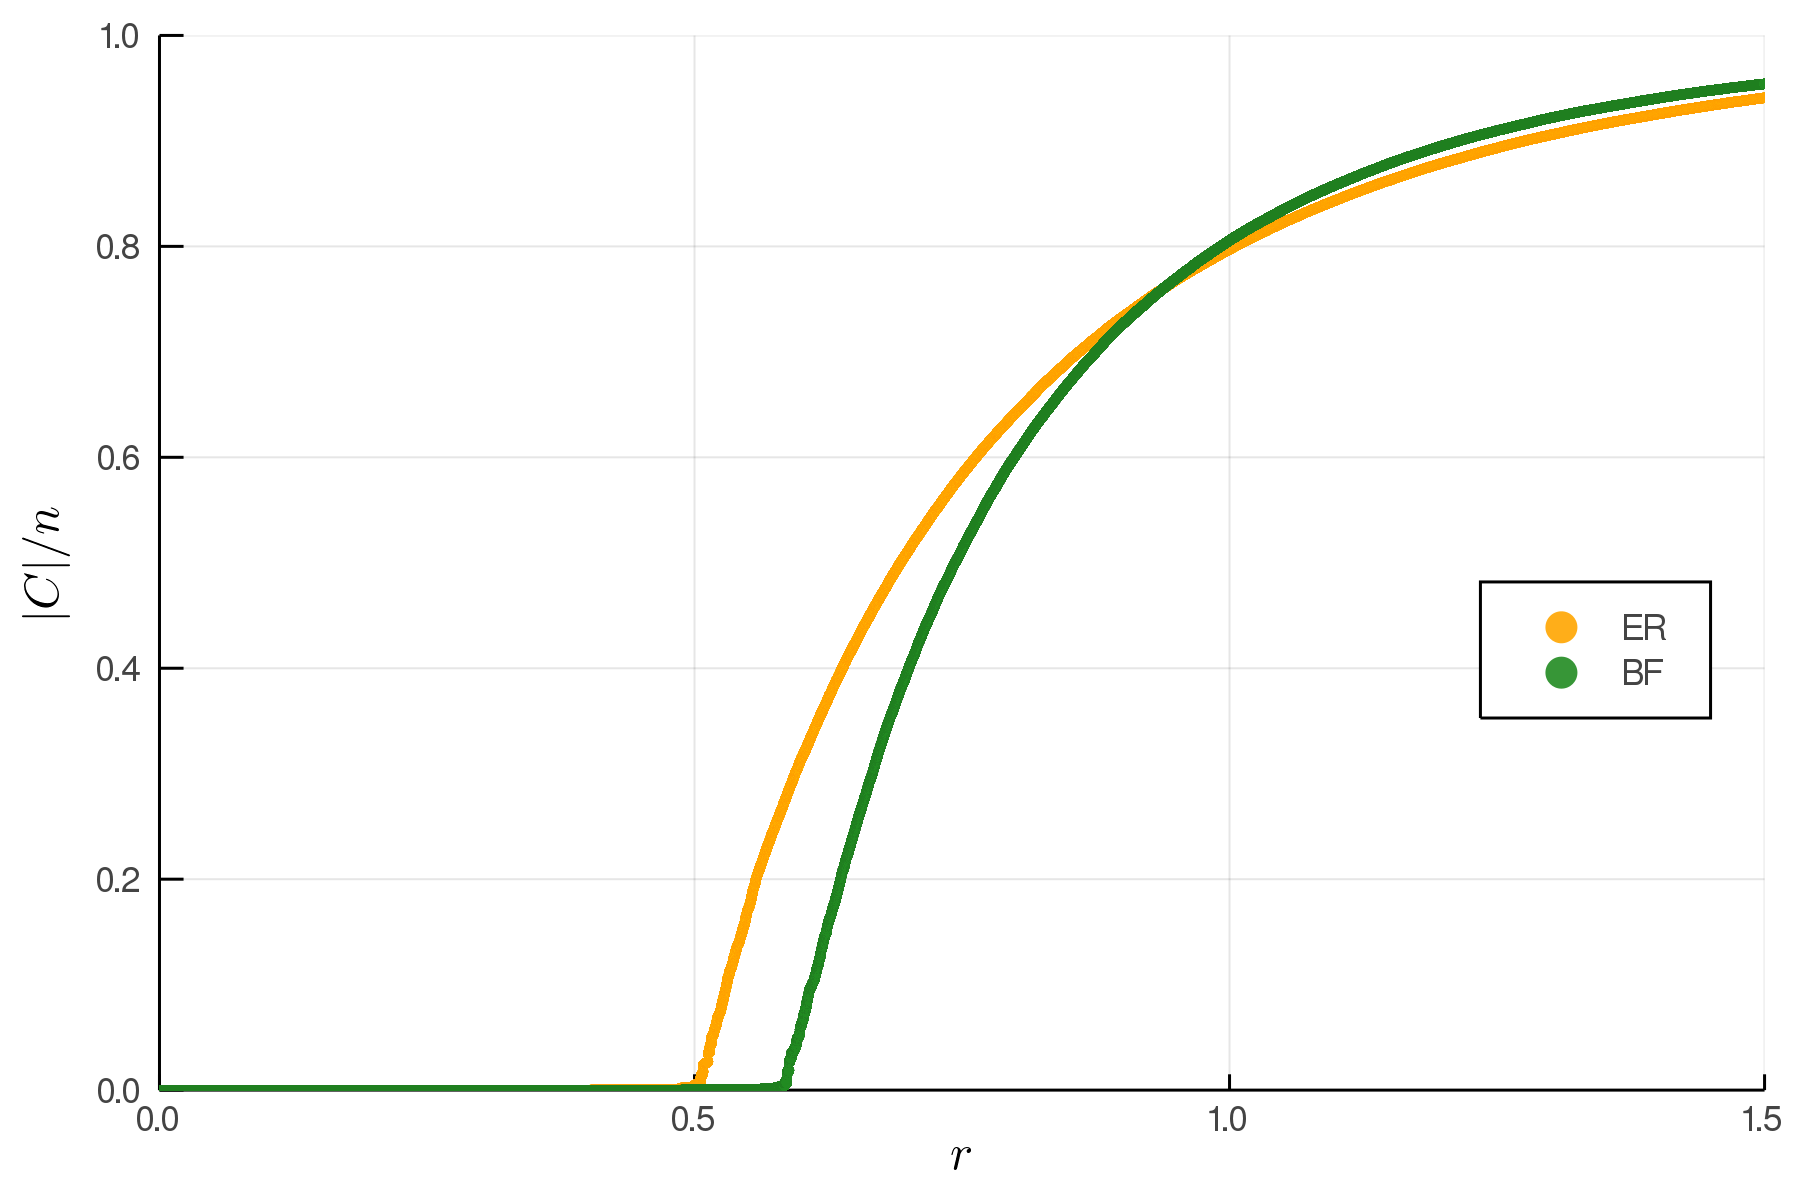
\includegraphics[width=350pt]{images/ER_BF_1e6_order_param.png}
	\caption{Bohman-Frieze Model Order Parameter, $n = 10^6$}
	\label{fig:ER_BF_transition}
\end{figure}









\subsection{A Discontinuous Transition?}
The first mention of explosive percolation appeared in 2009 in the paper "Explosive Percolation in Random Networks" \cite{Achlioptas} by Dimitris Achlioptas, Raissa M. D’Souza, and Joel Spencer, which will henceforth be referred to as Achlioptas et al.
In this paper they laid out a method of choosing edges called the product rule (PR).
At each step in the PR evolution process two edges are selected at random and evaluated based on the product of the cluster sizes that the edges would connect.
More specifically, if edge $e_1$ connects clusters $C_1$ and $C_2$ and edge $e_2$ connects clusters $C_3$ and $C_4$, then $e_1$ is accepted if $|C_1| \cdot |C_2| < |C_3| \cdot |C_4|$, otherwise $e_2$ is accepted.

This is illustrated in Fig. \ref{fig:edge_selection} where the first proposed edge $e_1$ would connect the blue cluster of size 5 to the red cluster of size 3 and the second proposed edge $e_2$ would connect the orange cluster of size 2 to the green cluster of size 4.
The product corresponding to $e_1$ is $5 \cdot 3 = 15$ whereas the product corresponding to $e_2$ is $2 \cdot 4 = 8$, so $e_1$ is rejected and $e_2$ accepted.
If we were looking at Fig. \ref{fig:edge_selection} from within the framework of the BF model with $K = 1$, then $e_1$ would be rejected and $e_2$ accepted even though both the orange and green clusters are of size greater than $K$.

\begin{figure}[H]
	\centering
	\includegraphics[width=200pt, clip]{images/edge_selection.png}
	\caption{Edge Selection}
	\label{fig:edge_selection}
\end{figure}

Fig. \ref{fig:ER_BF_PR_transition} shows the order parameters for the ER, BF, and PR models, making it clear just how drastically different the PR model transition is than in the ER/BF models.
As can be seen the order parameter remains near zero for much longer until the critical point $r_c \approx 0.888...$ \cite{Achlioptas}, which is much later than the critical point in the ER model of $r_c = 0.5$.
Not long after the critical point is reached the order parameter appears to jump up discontinuously, which was a surprising find.

\begin{figure}[H]
	\centering
	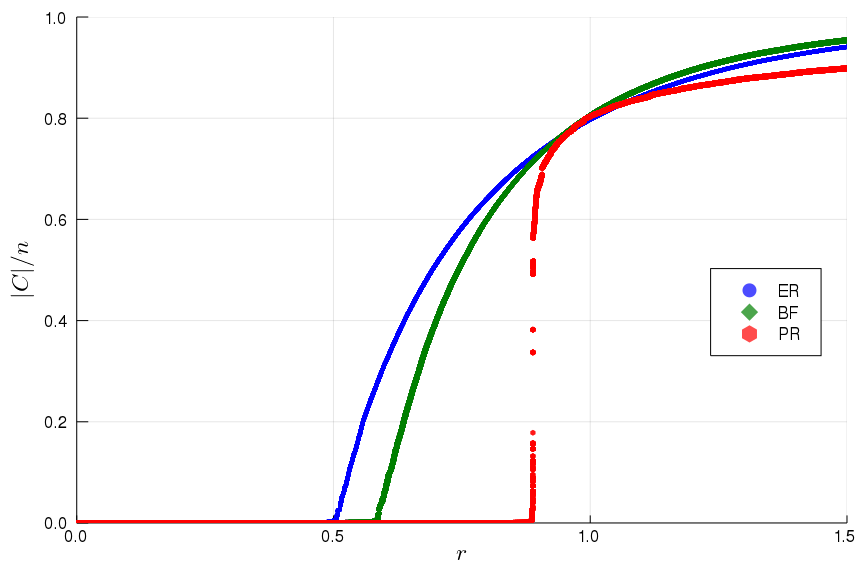
\includegraphics[width=350pt]{images/ER_BF_PR_1e6_order_param.png}
	\caption{Product Rule Model Order Parameter, $n = 10^6$}
	\label{fig:ER_BF_PR_transition}
\end{figure}

In their paper they analyzed the scaling behavior of their model, defining the quantity $\Delta := t_1 - t_0$, where $t_0$ is the last step where $C < n^{1/2}$ and $t_1$ is the first step where $C > 0.5n$.
$\Delta$ is linear in $n$ for continuous transitions (i.e. an extensive quantity), however, their analysis indicated otherwise that $\Delta < 2n^{2/3}$ and $\Delta / n^{2/3} \rightarrow 1$ in their simulations for sizes up to $6.4 \cdot 10^7$.
To arrive at these results they took an ensemble average of 50 different independent and identically distributed observations and fit a curve to determine the relation between $\Delta$ and $n$.
Their findings are illustrated in Fig. \ref{fig:achlioptas_plots}.
\cite{Achlioptas}

\begin{figure}[H]
	\centering
	\includegraphics[width=400pt]{images/achlioptas_plots.png}
	\caption{Achlioptas et al. Simulation Results, Source: \cite{Achlioptas}}
	\label{fig:achlioptas_plots}
\end{figure}

They ended their paper by saying: "We have demonstrated that small changes in edge formation have the ability to fundamentally alter the nature of percolation transitions. Our findings call for the comprehensive study of this phenomenon, and of its potential use in bringing phase transitions under control."
Indeed their message seemed to resonate, leading to a debate in the academic community about the nature and continuity of the transition.



\subsubsection{}
